\subsection{Initial Results}
As described in Section~\ref{sec:proposed_approach}, we conducted a series of initial experiments to evaluate the performance of various machine learning models on the prediction of major oxide compositions from our \gls{libs} dataset.
These experiments aimed to provide a preliminary assessment of the models' performance, allowing us to identify the most promising models for further evaluation and inclusion in our stacking ensemble.
All models were trained on the same preprocessed data using the Norm 3 preprocessing method described in Section~\ref{sec:norm3}.
This ensured that the models' performance could be evaluated under consistent and comparable conditions.

Table~\ref{tab:init_results} presents the results of these experiments, including the \gls{rmsep}, \gls{rmsecv}, standard deviation, and standard deviation of cross-validation prediction errors for each model across all oxides.
The means of each metric are also provided to give an overall indication of the models' performance.
Furthermore, we present an overview of these mean values in Figure~\ref{fig:init_results_rmses} to facilitate a visual comparison of the models' general performance.

The results indicate that the gradient boosting models, \gls{xgboost}, \gls{gbr}, and \gls{ngboost}, consistently perform well across all oxides, with \gls{xgboost} generally outperforming the other two gradient boosting models.
These models exhibit both low mean \gls{rmsep} and \gls{rmsecv} values, indicating high accuracy, as well as low standard deviation values, underscoring their robustness.
\gls{svr} is also among the top-performing models, with mean \gls{rmsep} and \gls{rmsecv} values close to those of \gls{xgboost} and low standard deviation values.

While usually outperformed by gradient boosting models and \gls{svr}, the ensemble models, \gls{rf} and \gls{etr}, also exhibit good performance.
The \gls{pls}, ridge, \gls{lasso}, and \gls{enet} models typically seem to perform worse than the other models, with higher mean \gls{rmsep} and \gls{rmsecv} values and higher standard deviation values.
We observe that \gls{enet} performs between ridge and \gls{lasso} in terms of both error and standard deviation, which aligns with expectations since \gls{enet} combines the regularization techniques of both models.

The \gls{cnn} and \gls{ann} models perform the worst across all oxides, exhibiting the highest mean \gls{rmsep} and \gls{rmsecv} values, as well as the highest standard deviation values.
This poor performance is further highlighted in Table~\ref{tab:relative_performance}, which shows the relative performance of each model compared to the best-performing model, \gls{xgboost}.
The table also includes the difference in performance relative to the next best model, with \gls{xgboost} serving as the baseline for comparison, assigned a relative performance of 100\%.
From this table, it is evident that the \gls{cnn} and \gls{ann} models experience significant drops in performance compared to the top-performing models.
While deep learning models such as these have the theoretical potential to perform well with \gls{libs} data, given their ability to learn complex patterns and relationships, the relatively small size of our dataset may limit their efficacy.
Furthermore, achieving optimal performance with these models necessitates extensive hyperparameter tuning, which involves exploring a vast space of potential configurations and design choices.
lthough methods for systematic hyperparameter optimization, as detailed in Section~\ref{sec:optimization_framework}, could be employed, the associated computational cost would be prohibitively high.
Additionally, there are numerous architectural design decisions and advanced techniques that could potentially enhance model performance, but their inclusion would significantly expand the scope of this study beyond feasible limits.
For these reasons, we decided to exclude the \gls{cnn} and \gls{ann} models from further experimentation.

Tables~\ref{tab:best_results} and \ref{tab:best_model_occurrences} list the best-performing model for each oxide and the frequency with which each model achieves top performance according to various metrics, respectively.
These tables are intended to provide an overview of model performance rather than to determine an overall 'winner by majority'.
Their purpose is to illustrate the general trends and behavior of different models across various metrics and oxides.
Although \gls{xgboost} and \gls{svr} appear the most frequently in Table~\ref{tab:best_model_occurrences}, this does not imply that they are the best models for every oxide.
The tables also demonstrates the importance of judging model performance per oxide.
For example, if one were to only consider the mean of the performance metrics, \gls{pls} would be considered among the worst performing models, as shown in Figure~\ref{fig:init_results_rmses}.
However, inspecting Table~\ref{tab:best_results} reveals that \gls{pls} exhibits the lowest \gls{rmsecv} and standard deviation of prediction errors for both \ce{MgO} and \ce{Na2O}.

This indicates that \gls{pls} is the most accurate and robust model for these oxides, underscoring the importance of evaluating model performance on a per-oxide basis, as discussed in Section~\ref{sec:proposed_approach}.
Moreover, for some oxides, multiple models perform similarly well, such as \gls{xgboost}, \gls{gbr}, and ridge for \ce{CaO}, which further emphasizes the need to leverage the strengths of multiple models.

To summarize, the initial results indicate that gradient boosting models, particularly \gls{xgboost}, demonstrated the most consistent and accurate performance across all oxides.
\gls{svr} also performed well, with similar accuracy and robustness to the gradient boosting models.
In contrast, deep learning models such as \gls{cnn} and \gls{ann} underperformed, likely due to the small dataset size and insufficient hyperparameter tuning.
Inspecting the model performances per oxide revealed that the best model varied depending on the oxide, and several models performed well for each oxide.
This emphasizes the need for further evaluation of model performances on a per-oxide basis to identify suitable configurations for our stacking ensemble approach, which aims to leverage the strengths of multiple models.

\begin{figure*}[h]
    \centering
    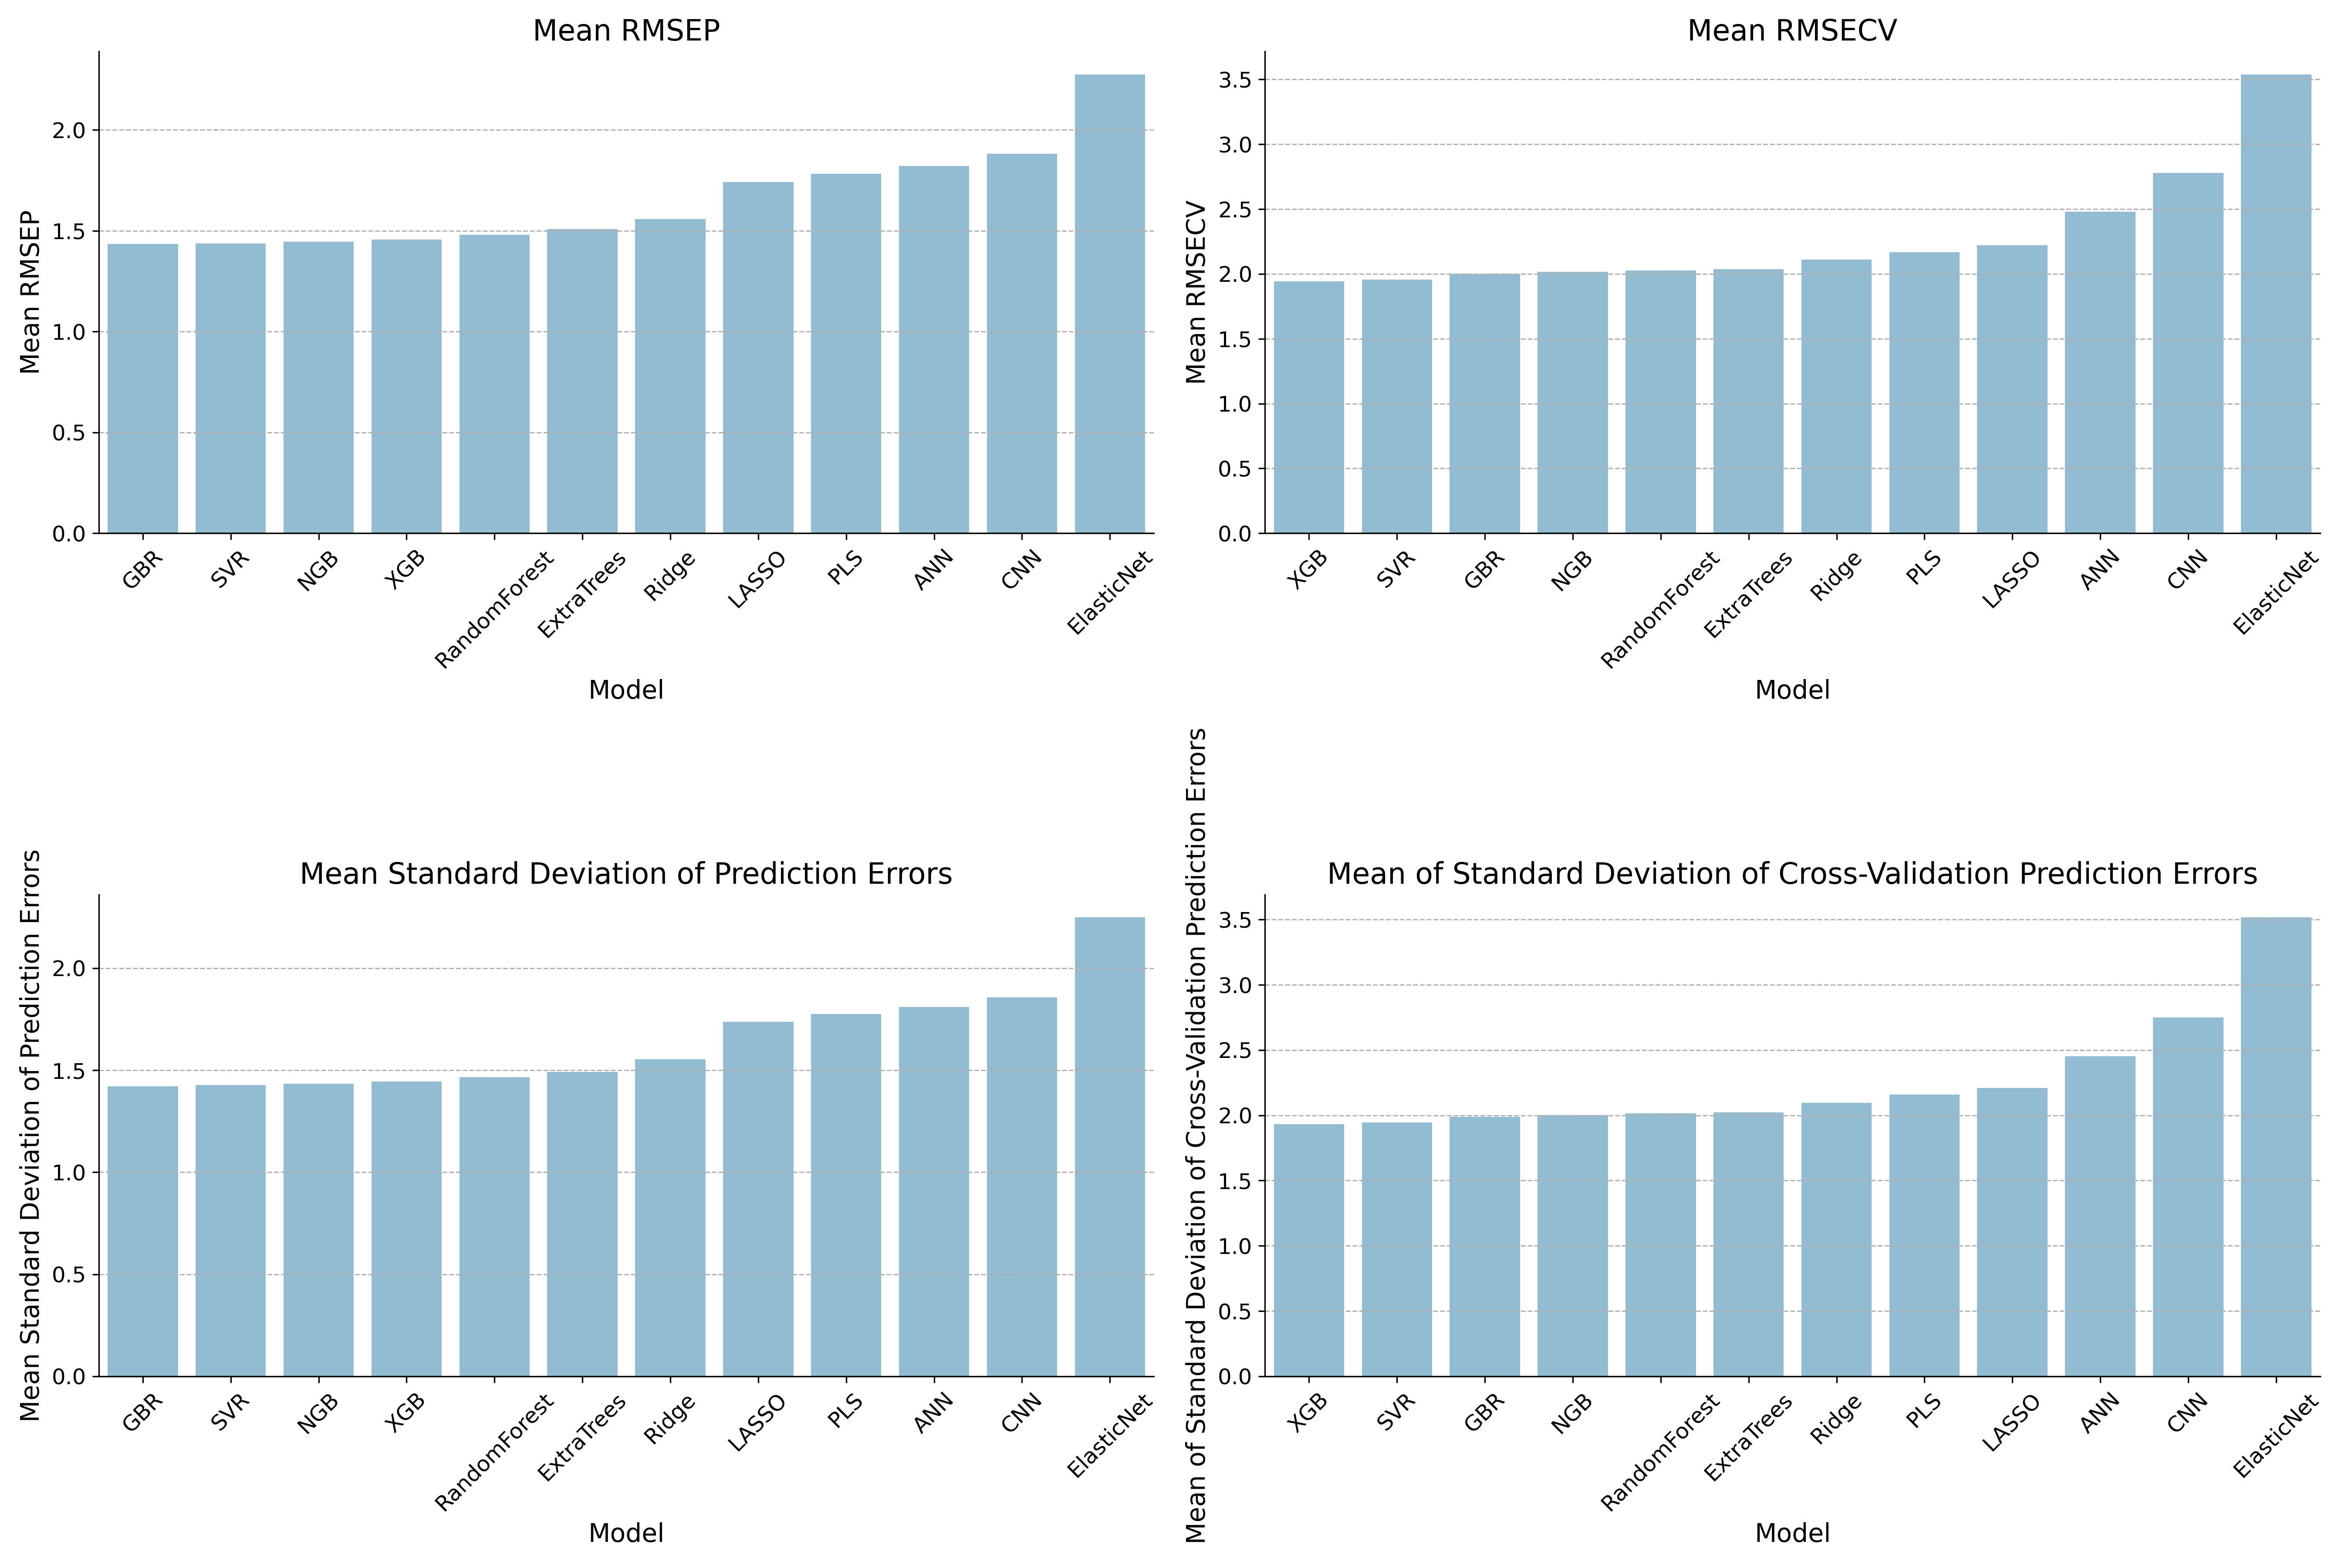
\includegraphics[width=\textwidth]{images/init_results_means.png}
    \caption{Mean \gls{rmsep}, \gls{rmsecv}, standard deviation of prediction errors, and standard deviation of cross-validation prediction errors for each model across all oxides.}
    \label{fig:init_results_rmses}
\end{figure*}

\begin{table}[ht]
\centering
\begin{tabularx}{\linewidth}{lrr}
\toprule
Model & Relative Performance (\%) & Diff. vs Next (\%) \\
\midrule
\gls{xgboost} & 100.00 & 0.85 \\
\gls{svr} & 100.85 & 2.22 \\
\gls{gbr} & 103.07 & 0.87 \\
\gls{ngboost} & 103.94 & 0.51 \\
\gls{rf} & 104.45 & 0.39 \\
\gls{etr} & 104.84 & 3.89 \\
Ridge & 108.74 & 2.92 \\
\gls{pls} & 111.66 & 2.73 \\
\gls{lasso} & 114.38 & 13.44 \\
\gls{ann} & 127.82 & 15.36 \\
\gls{cnn} & 143.18 & 39.18 \\
\gls{enet} & 182.36 & - \\
\bottomrule
\end{tabularx}
\caption{Relative performance of each model compared to the best performing model, and the difference in performance compared to the next best model.}
\label{tab:relative_performance}
\end{table}

\begin{table*}[]
\centering
\caption{Initial results for the different models and metrics.}
\resizebox{1\textwidth}{!}{%
\begin{tabular}{l|cccc|cccc|cccc}
Model & \multicolumn{4}{c}{Ridge} & \multicolumn{4}{c}{\gls{lasso}} & \multicolumn{4}{c}{\gls{enet}} \\
Metric & \multicolumn{1}{c}{RMSEP} & \multicolumn{1}{c}{RMSECV} & \multicolumn{1}{c}{Std. dev.} & \multicolumn{1}{c}{Std. dev. CV} & \multicolumn{1}{c}{RMSEP} & \multicolumn{1}{c}{RMSECV} & \multicolumn{1}{c}{Std. dev.} & \multicolumn{1}{c}{Std. dev. CV} & \multicolumn{1}{c}{RMSEP} & \multicolumn{1}{c}{RMSECV} & \multicolumn{1}{c}{Std. dev.} & \multicolumn{1}{c}{Std. dev. CV} \\
\hline
$\ce{SiO2}$ & 4.104 & 5.004 & 4.108 & 5.005 & 4.412 & 5.431 & 4.417 & 5.437 & 4.412 & 5.431 & 4.417 & 5.437 \\
$\ce{TiO2}$ & 0.424 & 0.470 & 0.413 & 0.469 & 0.398 & 0.556 & 0.389 & 0.555 & 0.398 & 0.556 & 0.389 & 0.555 \\
$\ce{Al2O3}$ & 2.322 & 2.913 & 2.324 & 2.888 & 2.349 & 3.063 & 2.352 & 3.044 & 2.349 & 3.063 & 2.352 & 3.044 \\
$\ce{FeOT}$ & 2.068 & 3.173 & 2.070 & 3.122 & 2.236 & 3.490 & 2.238 & 3.440 & 2.236 & 3.490 & 2.238 & 3.440 \\
$\ce{MgO}$ & 1.150 & 1.509 & 1.152 & 1.492 & 1.267 & 1.682 & 1.249 & 1.661 & 1.267 & 1.682 & 1.249 & 1.661 \\
$\ce{CaO}$ & 1.844 & 1.485 & 1.833 & 1.478 & 1.963 & 1.554 & 1.962 & 1.549 & 1.963 & 1.554 & 1.962 & 1.549 \\
$\ce{Na2O}$ & 0.632 & 1.089 & 0.633 & 1.084 & 0.625 & 1.114 & 0.616 & 1.111 & 0.588 & 1.085 & 0.587 & 1.082 \\
$\ce{K2O}$ & 0.651 & 0.668 & 0.645 & 0.668 & 0.638 & 0.859 & 0.629 & 0.856 & 0.638 & 0.859 & 0.629 & 0.856 \\
\hline
Mean & 1.649 & 2.039 & 1.647 & 2.026 & 1.736 & 2.219 & 1.732 & 2.207 & 1.731 & 2.215 & 1.728 & 2.203 \\
\hline
Model & \multicolumn{4}{c}{\gls{pls}} & \multicolumn{4}{c}{\gls{svr}} & \multicolumn{4}{c}{\gls{rf}} \\
Metric & \multicolumn{1}{c}{RMSEP} & \multicolumn{1}{c}{RMSECV} & \multicolumn{1}{c}{Std. dev.} & \multicolumn{1}{c}{Std. dev. CV} & \multicolumn{1}{c}{RMSEP} & \multicolumn{1}{c}{RMSECV} & \multicolumn{1}{c}{Std. dev.} & \multicolumn{1}{c}{Std. dev. CV} & \multicolumn{1}{c}{RMSEP} & \multicolumn{1}{c}{RMSECV} & \multicolumn{1}{c}{Std. dev.} & \multicolumn{1}{c}{Std. dev. CV} \\
\hline
$\ce{SiO2}$ & 4.141 & 5.701 & 4.145 & 5.693 & 3.552 & 4.908 & 3.555 & 4.908 & 3.715 & 5.304 & 3.699 & 5.292 \\
$\ce{TiO2}$ & 0.452 & 0.531 & 0.441 & 0.530 & 0.461 & 0.463 & 0.455 & 0.462 & 0.331 & 0.427 & 0.321 & 0.425 \\
$\ce{Al2O3}$ & 2.073 & 3.322 & 2.061 & 3.302 & 1.931 & 2.700 & 1.934 & 2.693 & 2.076 & 2.443 & 2.079 & 2.433 \\
$\ce{FeOT}$ & 3.222 & 3.117 & 3.221 & 3.114 & 1.823 & 2.847 & 1.814 & 2.809 & 2.091 & 3.091 & 2.073 & 3.053 \\
$\ce{MgO}$ & 1.106 & 1.296 & 1.103 & 1.296 & 0.789 & 1.426 & 0.785 & 1.419 & 0.911 & 1.742 & 0.904 & 1.731 \\
$\ce{CaO}$ & 1.937 & 1.813 & 1.923 & 1.792 & 1.626 & 1.532 & 1.594 & 1.508 & 1.765 & 1.503 & 1.754 & 1.499 \\
$\ce{Na2O}$ & 0.545 & 0.908 & 0.536 & 0.906 & 0.742 & 1.096 & 0.725 & 1.086 & 0.420 & 1.028 & 0.421 & 1.023 \\
$\ce{K2O}$ & 0.774 & 0.650 & 0.772 & 0.646 & 0.567 & 0.690 & 0.555 & 0.689 & 0.524 & 0.681 & 0.476 & 0.676 \\
\hline
Mean & 1.781 & 2.167 & 1.775 & 2.160 & 1.436 & 1.958 & 1.427 & 1.947 & 1.479 & 2.027 & 1.466 & 2.017 \\
\hline
Model & \multicolumn{4}{c}{\gls{ngboost}} & \multicolumn{4}{c}{\gls{gbr}} & \multicolumn{4}{c}{\gls{xgboost}} \\
Metric & \multicolumn{1}{c}{RMSEP} & \multicolumn{1}{c}{RMSECV} & \multicolumn{1}{c}{Std. dev.} & \multicolumn{1}{c}{Std. dev. CV} & \multicolumn{1}{c}{RMSEP} & \multicolumn{1}{c}{RMSECV} & \multicolumn{1}{c}{Std. dev.} & \multicolumn{1}{c}{Std. dev. CV} & \multicolumn{1}{c}{RMSEP} & \multicolumn{1}{c}{RMSECV} & \multicolumn{1}{c}{Std. dev.} & \multicolumn{1}{c}{Std. dev. CV} \\
\hline
$\ce{SiO2}$ & 4.112 & 5.071 & 4.081 & 5.010 & 3.576 & 4.995 & 3.479 & 4.922 & 3.953 & 4.898 & 3.926 & 4.876 \\
$\ce{TiO2}$ & 0.340 & 0.433 & 0.333 & 0.430 & 0.474 & 0.449 & 0.473 & 0.446 & 0.334 & 0.437 & 0.328 & 0.436 \\
$\ce{Al2O3}$ & 1.931 & 2.291 & 1.933 & 2.282 & 1.894 & 2.518 & 1.891 & 2.511 & 1.912 & 2.198 & 1.913 & 2.193 \\
$\ce{FeOT}$ & 1.588 & 3.561 & 1.590 & 3.530 & 1.594 & 3.069 & 1.596 & 3.068 & 1.848 & 3.020 & 1.838 & 3.002 \\
$\ce{MgO}$ & 0.849 & 1.578 & 0.845 & 1.574 & 0.964 & 1.766 & 0.960 & 1.763 & 0.905 & 1.781 & 0.901 & 1.771 \\
$\ce{CaO}$ & 1.740 & 1.610 & 1.723 & 1.602 & 1.768 & 1.468 & 1.769 & 1.468 & 1.765 & 1.467 & 1.749 & 1.457 \\
$\ce{Na2O}$ & 0.416 & 0.921 & 0.415 & 0.916 & 0.481 & 1.130 & 0.481 & 1.123 & 0.387 & 1.071 & 0.387 & 1.062 \\
$\ce{K2O}$ & 0.582 & 0.675 & 0.545 & 0.673 & 0.727 & 0.609 & 0.719 & 0.610 & 0.547 & 0.658 & 0.511 & 0.657 \\
\hline
Mean & 1.445 & 2.017 & 1.433 & 2.002 & 1.435 & 2.001 & 1.421 & 1.989 & 1.456 & 1.941 & 1.444 & 1.932 \\
\hline
Model & \multicolumn{4}{c}{\gls{etr}} & \multicolumn{4}{c}{\gls{ann}} & \multicolumn{4}{c}{\gls{cnn}} \\
Metric & \multicolumn{1}{c}{RMSEP} & \multicolumn{1}{c}{RMSECV} & \multicolumn{1}{c}{Std. dev.} & \multicolumn{1}{c}{Std. dev. CV} & \multicolumn{1}{c}{RMSEP} & \multicolumn{1}{c}{RMSECV} & \multicolumn{1}{c}{Std. dev.} & \multicolumn{1}{c}{Std. dev. CV} & \multicolumn{1}{c}{RMSEP} & \multicolumn{1}{c}{RMSECV} & \multicolumn{1}{c}{Std. dev.} & \multicolumn{1}{c}{Std. dev. CV} \\
\hline
$\ce{SiO2}$ & 3.995 & 5.230 & 3.970 & 5.225 & 4.664 & 7.025 & 4.670 & 6.981 & 4.662 & 6.061 & 4.626 & 6.046 \\
$\ce{TiO2}$ & 0.330 & 0.439 & 0.321 & 0.438 & 0.436 & 0.543 & 0.431 & 0.540 & 0.571 & 0.634 & 0.565 & 0.628 \\
$\ce{Al2O3}$ & 1.845 & 2.368 & 1.847 & 2.359 & 2.624 & 3.049 & 2.628 & 3.026 & 2.482 & 2.871 & 2.457 & 2.854 \\
$\ce{FeOT}$ & 2.144 & 3.299 & 2.126 & 3.257 & 2.534 & 3.836 & 2.497 & 3.748 & 2.588 & 4.584 & 2.521 & 4.488 \\
$\ce{MgO}$ & 0.906 & 1.755 & 0.895 & 1.738 & 1.315 & 1.818 & 1.300 & 1.768 & 1.292 & 2.892 & 1.280 & 2.857 \\
$\ce{CaO}$ & 1.837 & 1.515 & 1.831 & 1.510 & 1.799 & 1.633 & 1.772 & 1.634 & 2.009 & 2.142 & 2.008 & 2.099 \\
$\ce{Na2O}$ & 0.411 & 1.031 & 0.409 & 1.028 & 0.539 & 1.095 & 0.532 & 1.091 & 0.656 & 1.364 & 0.657 & 1.357 \\
$\ce{K2O}$ & 0.591 & 0.642 & 0.540 & 0.636 & 0.659 & 0.850 & 0.640 & 0.845 & 0.783 & 1.684 & 0.742 & 1.657 \\
\hline
Mean & 1.507 & 2.035 & 1.492 & 2.024 & 1.821 & 2.481 & 1.809 & 2.454 & 1.880 & 2.779 & 1.857 & 2.748 \\
\hline
\end{tabular}%
}
\label{tab:init_results}
\end{table*}


\begin{table*}[h]
\centering
\begin{minipage}{.7\textwidth}
  \centering
  \begin{tabular}{l|llll}
Oxide & RMSEP & RMSECV & Std. dev. & Std. dev. CV \\
\hline
$\ce{SiO2}$ & 3.552 (\gls{svr}) & 4.898 (\gls{xgboost}) & 3.479 (\gls{gbr}) & 4.876 (\gls{xgboost}) \\
$\ce{TiO2}$ & 0.330 (\gls{etr}) & 0.427 (\gls{rf}) & 0.321 (\gls{etr}) & 0.425 (\gls{rf}) \\
$\ce{Al2O3}$ & 1.845 (\gls{etr}) & 2.198 (\gls{xgboost}) & 1.847 (\gls{etr}) & 2.193 (\gls{xgboost}) \\
$\ce{FeOT}$ & 1.588 (\gls{ngboost}) & 2.847 (\gls{svr}) & 1.590 (\gls{ngboost}) & 2.809 (\gls{svr}) \\
$\ce{MgO}$ & 0.789 (\gls{svr}) & 1.296 (\gls{pls}) & 0.785 (\gls{svr}) & 1.296 (\gls{pls}) \\
$\ce{CaO}$ & 1.626 (\gls{svr}) & 1.467 (\gls{xgboost}) & 1.594 (\gls{svr}) & 1.457 (\gls{xgboost}) \\
$\ce{Na2O}$ & 0.387 (\gls{xgboost}) & 0.908 (\gls{pls}) & 0.387 (\gls{xgboost}) & 0.906 (\gls{pls}) \\
$\ce{K2O}$ & 0.524 (\gls{rf}) & 0.609 (\gls{gbr}) & 0.476 (\gls{rf}) & 0.610 (\gls{gbr}) \\
\hline
\end{tabular}%
\label{tab:best_results}

  \caption{Lowest metric and corresponding model for each oxide.}
  \label{tab:best_results}
\end{minipage}%
\hspace{0.03\textwidth}
\begin{minipage}{.25\textwidth}
  \centering
  \begin{table}[H]
\centering
\begin{tabular}{lc}
Model & Occurrences \\
\hline
\gls{xgboost} & 8 \\
\gls{svr} & 7 \\
\gls{etr} & 4 \\
\gls{rf} & 4 \\
\gls{pls} & 4 \\
\gls{gbr} & 3 \\
\gls{ngboost} & 2 \\
\end{tabular}
\caption{Occurrences of the best model for each oxide.}
\label{tab:best_model_occurrences}
\end{table}
\begin{tabular}{lc}
Model & Occurrences \\
\hline
\gls{xgboost} & 8 \\
\gls{svr} & 7 \\
\gls{etr} & 4 \\
\gls{rf} & 4 \\
\gls{pls} & 4 \\
\gls{gbr} & 3 \\
\gls{ngboost} & 2 \\
\end{tabular}
\label{tab:best_model_occurrences}

  \caption{Occurrences of the best model for each oxide.}
  \label{tab:best_model_occurrences}
\end{minipage}
\end{table*}
